\documentclass[class=report, crop=false, 12pt,a4paper]{standalone}
\usepackage{enumitem}
\usepackage{multicol}
\usepackage{graphicx}
\usepackage{float}
\usepackage{amsmath}
\usepackage{amssymb}
\usepackage{mathtools}
\usepackage{siunitx}
\usepackage{commath}
\usepackage{array}
\usepackage{natbib}
\usepackage{tikz}
\usepackage[a4paper,width=150mm,top=25mm,bottom=25mm]{geometry}
\allowdisplaybreaks
\setlength{\parindent}{0pt}
\begin{document}
\begin{center}
    19/01/2021
\end{center}
\section{Review on Thermodynamics}
\subsection{System, Surroundings and Boundary}
\textbf{Thermodynamic system} - An amount of matter “or” a region of space chosen for study \\
\textbf{Surroundings} - The region of space outside the arbitrary System boundary \\
\textbf{Boundary} - surface that separates the system from surrounding:
\begin{itemize}[noitemsep]
  \item Real or imaginary
  \item Massless
  \item Fixed (rigid tank) or movable (piston), flexible (balloon)
\end{itemize}
\begin{figure}[H]
  \centering
  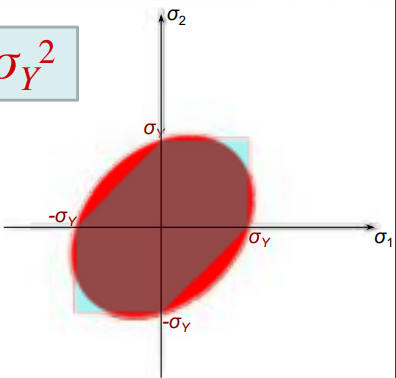
\includegraphics[width = 0.4 \textwidth]{../img/diagram92.png}
  \caption{}
\end{figure}
Identification of system and its surroundings is the most critical first step to begin thermodynamic analysis.
\subsection{System Classifications}
Different types of systems can be found, depending on whether work, heat or mass cross the system boundary.
\begin{table}[H]
  \centering
  \begin{tabular}{|c|c|c|c|c|}
  \hline
  \multicolumn{2}{|c|}{\textbf{Definition}} & \textbf{Work} & \textbf{Heat} & \textbf{Mass} \\ \hline
  \multicolumn{2}{|c|}{Isolated System}     & No            & No            & No            \\ \hline
  Closed System      & (Control Mass)       & Yes           & Yes           & No            \\ \hline
  Open System        & (Control Volume)     & Yes           & Yes           & Yes           \\ \hline
  \end{tabular}
\end{table}
\subsection{Thermodynamic Properties - Extensive vs. Intensive}
Extensive properties are additive (i.e. depending on size/mass of system)
\begin{itemize}[noitemsep]
  \item U: internal energy \ [kJ] 
  \item H: enthalpy \ [kJ] 
  \item S: entropy \ [kJ/K]
  \item V: volume \ [$\si{\metre\cubed}$]
\end{itemize}
Intensive properties are non-additive (i.e. independent of size/mass of system)
\begin{itemize}[noitemsep]
  \item T: temperature \ [K] 
  \item h: specific enthalpy \ [kJ/kg]
  \item P: pressure \ [Pa] 
  \item s: specific entropy \ [kJ/(kg K)]
  \item x: quality \ [-] 
  \item v: specific volume \ [$\si{\metre\cubed}$/kg]
  \item u: specific internal energy \ [kJ/kg] 
  \item $\rho$: density \ [kg/$\si{\metre\cubed}$]
\end{itemize}
Extensive properties per unit mass or mole are called specific properties, which become intensive properties.
\subsection{State, Equilibrium State, Steady State}
\textbf{State} of a system is the condition characterized by a given set of properties, as well as their distributions in space. For a simple system of pure homogeneous substance, the state is uniquely specified by just two properties such as T and P or V and S. \\\\
\textbf{Thermodynamic equilibrium (state)} implies that a system state cannot change in the absence of unbalanced driving \textbf{forces”} between the system and surroundings. It requires the following equilibrium within the system: 
\begin{itemize}[noitemsep]
  \item Thermal equilibrium (constant temperature)
  \item Mechanical equilibrium (no pressure difference without gravity)
  \item Chemical equilibrium (no chemical reactions)
  \item Phase equilibrium (no phase change)
\end{itemize}
\textbf{Steady state} requires none of its properties changes with time, but within the system, the properties at different locations can be different.
\section{Ideal Gas}
Ideal gas is an imaginary substance whose properties satisfy the following state equation: 
\begin{gather}
  PV = nRT
\end{gather}
Some Assumptions:
\begin{itemize}[noitemsep]
  \item No molecular volume: molecules do not occupy space
  \item No intermolecular forces: intermolecular force can be neglected
\end{itemize}
These assumptions are not always valid. Substances may be treated as ideal gases for engineering applications at sufficiently low pressure and high temperatures (i.e. low density)
\subsection{Ideal Gas Equation of State}
On a molar basis:
\begin{gather}
  PV = NR_uT \\[5pt]
  P\overline{v} = R_uT
\end{gather}
On a mass basis:
\begin{gather}
  PV = mRT \\[5pt] 
  Pv = RT
\end{gather}
Where:
\begin{itemize}[noitemsep]
  \item $N$ = number of moles of gas \ [kmol]
  \item $T$ = absolute temperature \ [K]
  \item $R_u$ = universal gas constant $= 8.314 \ [\si{\kilo\joule\per\kilo\mole\per\kelvin}]$
  \item $V$ = volume \ $[\si{\metre\cubed}]$
  \item $v$ = specific volume \ $[\si{\metre\cubed\per\kilogram}]$; \ \ $\overline{v} \ \ [\si{\metre\cubed\per\kilo\mole}]$
  \item $R$ = $R_u/M$ = specific gas constant \ [kJ/kgK]
  \item $M$ = molecular weight of gas \ [kg/kmol]
\end{itemize}
\subsection{Limitations on Ideal Gas EoS}
\begin{itemize}
  \item Usually good for air, N$_2$, O$_2$, H$_2$, He, Ar, Ne at low pressures and high temperatures (less than $1\%$ error)
  \item Works well for water vapour below $10\si{\kilo\pascal}$ irrespective of temperature (less than $0.1\%$ error)
  \item Fails close to critical point and saturated vapour line
  \item Definitely not applicable for water vapour in steam power plants owing to very high pressures
\end{itemize}
\section{Ideal Gas Mixtures}
Aim: To develop rules for evaluating the properties of gas mixtures using the properties of individual gases (called components or constituents). \\\\
Assumptions:
\begin{itemize}[noitemsep]
  \item Each gas in the mixture behaves like an ideal gas.
  \item The overall mixture behaves like an ideal gas.
\end{itemize}
Examples:
\begin{itemize}[noitemsep]
  \item Air
  \item Syngas
  \item Exhaust gases of a combustion process
\end{itemize}
\section{Composition of Mixtures}
State of a mixture is fully determined by:
\begin{itemize}
  \item Composition: mass $m_i$ or number of moles $n_1$ of each component;
  \item Two independent intensive properties (such as $p$ and $T$ or $v$ and $T$).  
\end{itemize}
Mass $m_i$, number of moles $n_i$ and molecular weight $M_i$ of each component $i$ are related by:
\begin{gather}
  n_i = \frac{m_i}{M_i}
\end{gather}
Mass fraction, $x_i$:
\begin{gather}
  x_i = \frac{m_i}{m} \longrightarrow \sum_{i=1}^{k}x_i = 1
\end{gather}
\begin{center}
  Mass fraction based analysis $\longrightarrow$ gravimetric analysis
\end{center}
Mole fraction, $y_i$:
\begin{gather}
  y_i = \frac{n_i}{n} \longrightarrow \sum_{i=1}^{k}y_i = 1
\end{gather}
\begin{center}
  Molar analysis $\longrightarrow$ volumetric analysis
\end{center}
Apparent or Average molecular weight, $M$:
\begin{gather}
  M = \frac{m}{n} = \frac{\sum_{i=1}^{k}m_i}{n} = \frac{\sum_{i=1}^{k}n_i M_i}{n} = \sum_{i=1}^{k}y_i M_i
\end{gather}
Total mass of the mixture: 
\begin{gather}
  m = m_1 + m_2 + \dots + m_k = \sum_{i=1}^{k}m_i
\end{gather}
Mass fraction of $i^{\text{th}}$ component:
\begin{gather}
  x_i = \frac{m_i}{m} \longrightarrow \sum_{i=1}^{k}x_i = 1
\end{gather}
Total number of moles:
\begin{gather}
  n = n_1 + n_2 + \dots + n_k = \sum_{i=1}^{k}n_i
\end{gather}
Mole fraction of $i^{\text{th}}$ component:
\begin{gather}
  y_i = \frac{n_i}{n} \longrightarrow \sum_{i=1}^{k}y_i = 1
\end{gather}
Molar mass: 
\begin{gather}
  M_i = \frac{m_i}{n_i} \ \text{(single component)} \ \ \ \ \ M = \frac{m}{n} \ \text{(mixture)} \\[5pt]
  m = n_1M_1 + n_2M_2 + \dots + n_kM_k = nM
\end{gather}
\subsection{Composition of Air}
In practical calculations, air can be assumed to consist of $21\%$ oxygen and $79\%$ nitrogen by volume.
\begin{table}[]
  \centering
  \begin{tabular}{|c|c|c|c|c|}
  \hline
  Constituent & Mass Fraction $x_i$ & Molar Mass $M_i$                                                               & \begin{tabular}[c]{@{}c@{}}Moles $n_i$ \\ per kg of mixture\end{tabular}         & Mole Fraction $y_i$ \\ \hline
  O$_2$       & 0.232               & 32                                                                             & 0.00725                                                                          & 0.210               \\ \hline
  N$_2$       & 0.756               & 28.01                                                                          & 0.02699                                                                          & 0.781               \\ \hline
  Ar          & 0.012               & 39.94                                                                          & 0.00300                                                                          & 0.009               \\ \hline
  Air         & 1                   & \begin{tabular}[c]{@{}c@{}}28.96 \\ $\si{\kilogram\per\kilo\mole}$\end{tabular} & \begin{tabular}[c]{@{}c@{}}0.03454 \\ $\si{\kilo\mole\per\kilogram_{air}}$\end{tabular} & 1.0                 \\ \hline
  \end{tabular}
\end{table}
\begin{gather}
  M_{air} = \frac{m_{air}}{n_{air}} = \frac{1}{0.03454} = 28.96 \si{\kilogram\per\kilo\mole}
\end{gather}
\section{P-v-T Relationships of Ideal Gas Mixtures}
\subsection{Dalton's Law}
\begin{figure}[H]
  \centering
  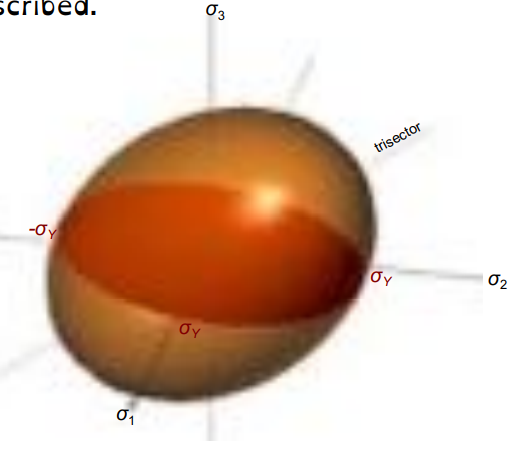
\includegraphics[width = 0.4 \textwidth]{../img/diagram93.png}
  \caption{}
\end{figure}
The pressure of a gas mixture is equal to the sum of the pressures each gas would exert if it existed alone at the mixture temperature and volume.
\begin{figure}[H]
  \centering
  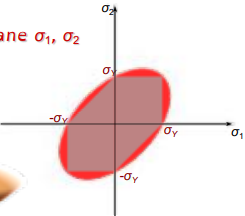
\includegraphics[width = 0.7 \textwidth]{../img/diagram94.png}
  \caption{}
\end{figure}
Ideal gas law and the universal gas constant are, respectively:
\begin{gather}
  p_iV = n_i\overline{R}T \\[5pt]
  \overline{R} = R_u = R_0 = 8.314 \si{\kilo\joule\per\kilo\mole\per\kelvin}
\end{gather}
The pressure of each component occupying the whole volume of the mixture at the same mixture temperature is a \textbf{partial pressure}:
\begin{gather}
  p_i = \frac{n_i \overline{R} T}{V} \\[5pt]
  p = \frac{n \overline{R} T}{V} \\[5pt]
  \frac{p_i}{p} = \frac{n_i}{n} = y_i \\[5pt]
  p_i = y_ip \\[5pt]
  \sum_{i=1}^{j}p_i = \sum_{i=1}^{j}y_ip = p\sum_{i=1}^{j}y_i = p
\end{gather}
\subsection{Amagat’s Law}
\begin{figure}[H]
  \centering
  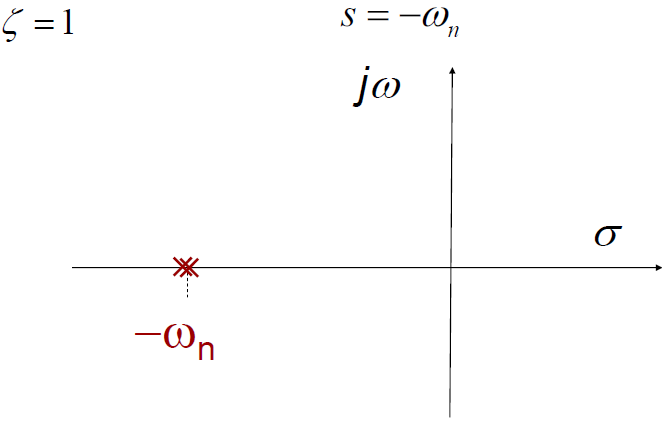
\includegraphics[width = 0.4 \textwidth]{../img/diagram95.png}
  \caption{}
\end{figure}
The volume of a gas mixture is equal to the sum of the volumes each gas would occupy if it existed alone at the mixture temperature and pressure.
\begin{figure}[H]
  \centering
  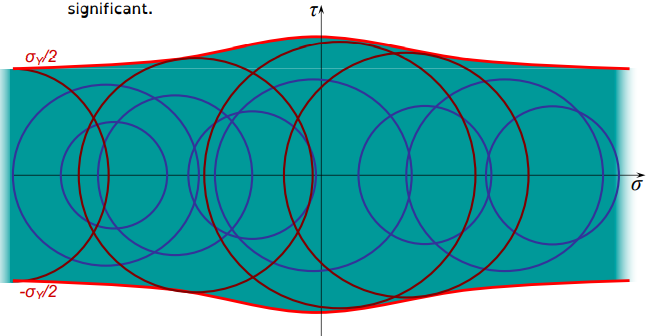
\includegraphics[width = 0.65 \textwidth]{../img/diagram96.png}
  \caption{}
\end{figure}
Ideal gas law and the universal gas constant are, respectively:
\begin{gather}
  pV_i = n_i\overline{R}T \\[5pt]
  \overline{R} = R_u = R_0 = 8.314 \si{\kilo\joule\per\kilo\mole\per\kelvin}
\end{gather}
The volume occupied by each component at the same pressure $p$ and temperature $T$ of the mixture is a \textbf{partial volume}: 
\begin{gather}
  V_i = \frac{n_i \overline{R} T}{p} \\[5pt]
  V = \frac{n \overline{R} T}{p} \\[5pt]
  \frac{V_i}{V} = \frac{n_i}{n} = y_i \\[5pt]
  V_i = y_iV \\[5pt]
  \sum_{i=1}^{j}V_i = \sum_{i=1}^{j}y_iV = V\sum_{i=1}^{j}y_i = V
\end{gather}
\section{Properties of Ideal Gas Mixtures}
Extensive properties $U$, $H$, $S$ and intensive properties $u$, $h$, $s$:
\subsubsection{Internal Energy}
\begin{gather}
  U = U_1 + U_2 + \dots + U_k = \sum_{i=1}^{k}U_i \\[5pt]
  U = m_1u_1 + m_2u_2 + \dots + m_ku_k = \sum_{i=1}^{k}m_iu_i = mu \\[5pt]
  U = n_1\overline{u_1} + n_2\overline{u_2} + \dots + n_k\overline{u_k} = \sum_{i=1}^{k} n_i\overline{u_1} = n\overline{u} \\[5pt]
  u = \sum_{i=1}^{k} x_i u_i \ \ \si{\kilo\joule\per\kilogram} \\[5pt]
  \overline{u} = \sum_{i=1}^{k} y_i \overline{u_i} \ \ \si{\kilo\joule\per\kilo\mole}
\end{gather}
\subsubsection{Enthalpy}
\begin{gather}
  H = H_1 + H_2 + \dots + H_k = \sum_{i=1}^{k}H_i \\[5pt]
  H = m_1h_1 + m_2h_2 + \dots + m_kh_k = \sum_{i=1}^{k}m_ih_i = mh \\[5pt]
  H = n_1\overline{h_1} + n_2\overline{h_2} + \dots + n_k\overline{h_k} = \sum_{i=1}^{k} n_i\overline{h_1} = n\overline{h} \\[5pt]
  h = \sum_{i=1}^{k} x_i h_i \ \ \si{\kilo\joule\per\kilogram} \\[5pt]
  \overline{h} = \sum_{i=1}^{k} y_i \overline{h_i} \ \ \si{\kilo\joule\per\kilo\mole}
\end{gather}
\subsubsection{Entropy}
\begin{gather}
  S = S_1 + S_2 + \dots + S_k = \sum_{i=1}^{k}S_i \\[5pt]
  S = m_1s_1 + m_2s_2 + \dots + m_ks_k = \sum_{i=1}^{k}m_is_i = ms \\[5pt]
  S = n_1\overline{s_1} + n_2\overline{s_2} + \dots + n_k\overline{s_k} = \sum_{i=1}^{k} n_i\overline{s_1} = n\overline{s} \\[5pt]
  s = \sum_{i=1}^{k} x_i s_i \ \ \si{\kilo\joule\per\kilogram} \\[5pt]
  \overline{s} = \sum_{i=1}^{k} y_i \overline{s_i} \ \ \si{\kilo\joule\per\kilo\mole}
\end{gather}
For all extensive (depending on system size) properties:
\begin{gather}
  A = ma = n\overline{a} = \sum_{i=1}^{k}A_i = \sum_{i=1}^{k}m_i a_i = \sum_{i=1}^{k}n_1\overline{a_i}
\end{gather}
For all specific ($u$, $h$, $s$, $V$, $\phi$, $\psi$) properties: 
\begin{gather}
  a = \sum_{i=1}^{k}x_i a_i \\[5pt]
  \overline{a} = \sum_{i=1}^{k}y_i \overline{a_i}
\end{gather}
\subsection{Change in Properties}
Given:
\begin{gather}
  U = \sum_{i=1}^{k}m_i u_i
\end{gather}
Differentiation:
\begin{gather}
  \dif U = \dif\left(\sum_{i=1}^{k}m_i u_i\right) = \sum_{i=1}^{k}\dif\ (m_i u_i) \\[5pt]
  \dif U = \sum_{i=1}^{k}m_i\dif u_i + \sum_{i=1}^{k}u_i\dif m_i
\end{gather}
Change in mixture properties are due to 2 parts:
\begin{itemize}[noitemsep]
  \item changing component property $\longrightarrow \dif u_i$
  \item changing composition $\longrightarrow \dif m_i$
\end{itemize}
For non-reacting mixture, fixed composition $\longrightarrow \dif m_i = 0$. Hence:
\begin{gather}
  \dif U = \sum_{i=1}^{k}m_i\dif u_i \\[5pt]
  \dif u = \sum_{i=1}^{k}x_i\dif u_i
\end{gather}
In general:
\begin{gather}
  \dif A = \sum_{i=1}^{k}m_i \dif a_i \\[5pt]
  \dif a = \sum_{i=1}^{k}x_i \dif a_i
\end{gather}
\subsection{Specific Heats of Ideal Gas Mixture}
\subsubsection{Evaluating $C_v$ and $C_p$ of the mixture (volumetric analysis)}
Given:
\begin{gather}
  \overline{u} = \sum_{i=1}^{k}y_i\overline{u_i} \ \ \ \ \ \text{and} \ \ \ \ \ \overline{h} = \sum_{i=1}^{k}y_i\overline{h_i}
\end{gather}
Differentiation with respect to temperature leads to:
\begin{gather}
  \overline{c_v} = \sum_{i=1}^{k}y_i\overline{c}_{v,i} \ \ \ \ \ \text{and} \ \ \ \ \ \overline{c_p} = \sum_{i=1}^{k}y_i\overline{c}_{p,i}
\end{gather}
The specific ratio of heats of the mixture:
\begin{gather}
  \gamma = \frac{\overline{c_p}}{\overline{c_v}}
\end{gather}
\subsubsection{Evaluating $C_v$ and $C_p$ of the mixture (gravimetric analysis)}
Define specific heats for single component $i$ as:
\begin{gather}
  \dif u_i = c_{v,i}\dif T_i \ \ \ \ \ \text{and} \ \ \ \ \ \dif h_i = c_{p,i}\dif T_i
\end{gather}
For equilibrium conditions:
\begin{gather}
  \dif T_i = \dif T \\[5pt]
  \dif u = \sum_{i=1}^{k}x_i c_{v,i}\dif T \ \ \ \ \ \text{and} \ \ \ \ \ \dif h = \sum_{i=1}^{k}x_i c_{p,i}\dif T
\end{gather}
Also:
\begin{gather}
  \dif u = c_v\dif T \ \ \ \ \ \text{and} \ \ \ \ \ \dif h = c_p\dif T
\end{gather}
Therefore:
\begin{gather}
  c_v = \sum_{i=1}^{k}x_i c_{v,i} \ \ \ \ \ \text{and} \ \ \ \ \ c_p = \sum_{i=1}^{k}x_i c_{p,i}
\end{gather}
\subsection{Change in Properties of Mixture (non-reacting)}
\begin{figure}[H]
  \centering
  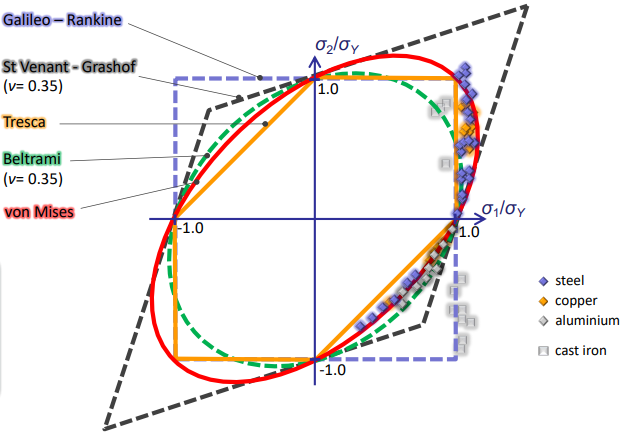
\includegraphics[width = 0.45 \textwidth]{../img/diagram97.png}
  \caption{}
\end{figure}
\begin{gather}
  U_2 - U_1 = \sum_{i=1}^{j}n_i\left[\overline{u}_i(T_2) - \overline{u}_i(T_1)\right] \\[5pt]
  \Delta\overline{u} = \sum_{i=1}^{j}y_i\left[\overline{u}_i(T_2) - \overline{u}_i(T_1)\right] \\[15pt]
  H_2 - H_1 = \sum_{i=1}^{j}n_i\left[\overline{h}_i(T_2) - \overline{h}_i(T_1)\right] \\[5pt]
  \Delta\overline{h} = \sum_{i=1}^{j}y_i\left[\overline{h}_i(T_2) - \overline{h}_i(T_1)\right] \\[15pt]
  S_2 - S_1 = \sum_{i=1}^{j}n_i\left[\overline{s}_i(T_2,p_{i2}) - \overline{s}_i(T_1,p_{i1})\right] \\[5pt]
  \Delta\overline{s} = \sum_{i=1}^{j}y_i\left[\overline{s}_i(T_2,p_{i2}) - \overline{s}_i(T_1,p_{i1})\right]
\end{gather}
Changes in mixture properties are written in terms of the respective property changes of the components, weighted by the mole fraction. \\\\
Changes in properties for component $i$ can be evaluated by:
\begin{itemize}[noitemsep]
  \item Either integration of the relevant equations or
  \item Tabulation of ideal gas properties 
\end{itemize}
\subsection{Change in Entropy of Ideal Gas Mixtures}
At fixed composition:
\begin{gather}
  \dif s = \sum_{i=1}^{k}x_i \dif s_i
\end{gather}
For an ideal gas mixture:
\begin{gather}
  \dif s = c_p\frac{\dif T}{T} - R\frac{\dif p}{p} \\[5pt]
  \Delta s = \int_{T_1}^{T_2}c_p\frac{\dif T}{T} - R\ln\left(\frac{p_2}{p_1}\right) \\[5pt]
  \Delta s = s_2^\circ - s_1^\circ - R\ln\left(\frac{p_2}{p_1}\right)
\end{gather}
Where:
\begin{gather}
  c_p = \sum_{i=1}^{k}x_i c_{p,i} \ \ \ \ \ \text{and} \ \ \ \ \ R = \frac{R_u}{M}
\end{gather}
For constant specific heat:
\begin{gather}
  \Delta s = c_p\ln\left(\frac{T_2}{T_1}\right) - R\ln\left(\frac{p_2}{p_1}\right)
\end{gather}
Then:
\begin{gather}
  \Delta s = \sum_{i=1}^{k}x_i \Delta s_i^\circ - \sum_{i=1}^{k}x_i R_i \ln\left(\frac{p_{i,2}}{p_{i,1}}\right)
\end{gather}
For constant specific heat:
\begin{gather}
  \Delta s = \sum_{i=1}^{k}x_i c_{p,i}\ln\left(\frac{T_2}{T_1}\right) - \sum_{i=1}^{k}x_i R_i \ln\left(\frac{p_{i,2}}{p_{i,1}}\right)
\end{gather}
On a molar basis:
\begin{gather}
  \Delta\overline{s} = \sum_{i=1}^{k}y_i \Delta \overline{s}_i^\circ - \sum_{i=1}^{k}y_i R_u \ln\left(\frac{p_{i,2}}{p_{i,1}}\right)
\end{gather}
\end{document}